\chapter{Technology of ice reservoirs}

AIRs are a natural evolution of Ladakh's agricultural system. They can be related to traditional water
harvesting technologies like the {\it zing}, which are small tanks where meltwater is collected through the use
of an intricate network of channels. The mountain oases of the Hindu Kush and Karakoram ranges
have similar irrigation networks \citep{nusserLocalKnowledgeGlobal2016}.

\begin{figure}[t]
\centering
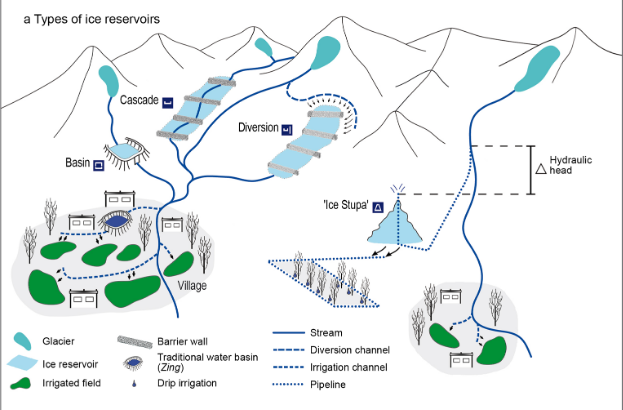
\includegraphics[width=12cm]{Figures/AIR_designs.png}

\caption{Adapted from: \cite{nusserSociohydrologyArtificialGlaciers2019}}

\label{fig:AIRdesigns}
\end{figure}

\section{Ice terraces}


\begin{figure}[t]
\centering
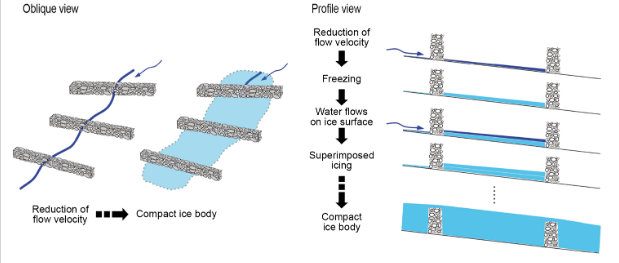
\includegraphics[width=12cm]{Figures/IT_science.png}

\caption{ The process of ice accumulation for ice terraces Adapted from:
\cite{nusserSociohydrologyArtificialGlaciers2019}}

\label{fig:ITscience}
\end{figure}

Ice terraces are the oldest form of AIRs \citep{norphelArtificialGlacierHigh2009}. Usually situated below the
glaciers at elevations where snowmelt starts end of March, these structures facilitate the freezing of stream
water during winter at selected sites, usually shaded by surrounding mountains. Chewang Norphel, a well known
engineer of the Leh Nutrition Project, introduced this practice to Ladakh in the 1980s and 1990s
\citep{vinceGlacierMan2009}.

\subsection{Construction strategy}

There are four distinct types of ice terraces with site-specific modifications as shown in Fig.
\ref{fig:AIRdesigns}: the first type is built as cascades on perennial streams. A series of loose rock walls in
the river bed reduce reduces flow velocity, but still lets water pass through. Such cascades allow flowing water
to freeze on exposed surfaces and form superimposed ice layers when temperatures drop. 

The second type diverts water from streams with higher flow velocity to small side valleys, shaded by
surrounding mountains. This design allows to integrate higher slope positions for additional ice formation. It
consists of a series of partially cemented stone walls across the stream bed. Their dimensions are adjusted
based on the valley topography. The water for the ice terrace is obtained through a long diversion channel. 

The third type is a basin structure, resembling the traditional {\it zing} form of water storage, but located
above the cultivated fields.

\subsection{Application}

\begin{figure}[t]
\centering
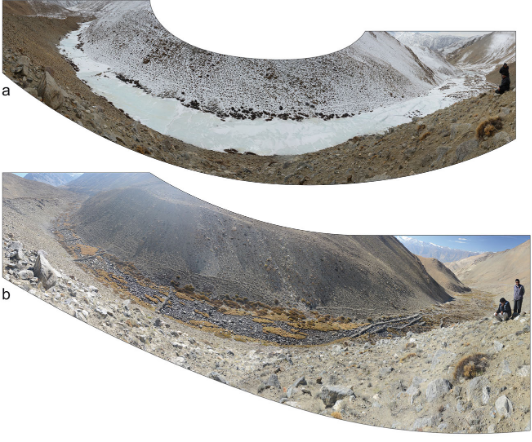
\includegraphics[width=12cm]{Figures/IT_example.png}

\caption{Ice terrace of Phuktse, viewpoint 4430 m. (a) February 2014 (b) October 2014 Adapted from: \cite{nusserSociohydrologyArtificialGlaciers2019}}

\label{fig:ITexample}
\end{figure}

Over the past 30 years, 14 ice terraces have been constructed in central Ladakh, located in tributary valleys of
the Indus. The oldest ice terrace was of the form cascades in Ladakh was built in 1987 at a favourable location
between 4290 and 4640 $m$ in Phuktse. However, according to oral history and Corona imagery from 1969, the first ice
terrace of this design type are older than 50 years and can be found in Phuktse and Igoo. In February 2014,
Phuktse built a successful cascade with an almost continuous stretch of ice (Fig.).


\subsection{Drawbacks}

However, the location requirements and the construction cost of ice terraces were prohibitive for widespread
adoption. 


\section{Ice stupas}

\begin{figure}[t]
\centering
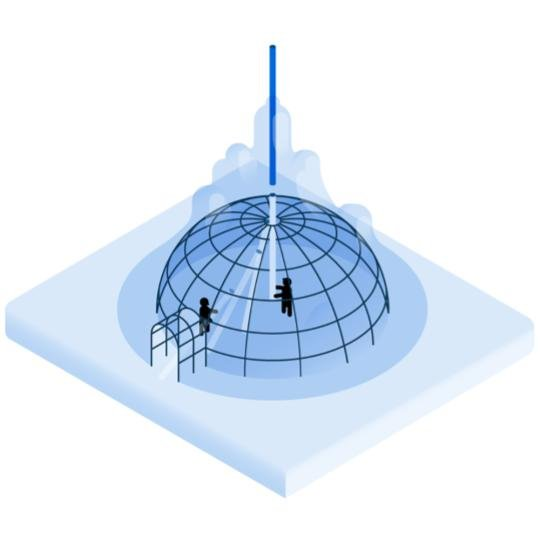
\includegraphics[width=12cm]{Figures/IS_science.jpg}

\caption{ The process of ice accumulation for ice stupas. Diagram by: Francesco Muzzi }

\label{fig:ISscience}
\end{figure}

This prompted the invention of Ice stupas by Sonam Wangchuk in 2013 \ref{wangchukIceStupaArtificial2014}. Due to
their shape, Ice stupas could be built adjacent to the irrigated plantations. It was also relatively cheaper. A
typical Ice stupa just requires a fountain nozzle mounted on a supply pipeline. The water source is usually a
spring or a glacial stream. Due to the altitude difference between the pipeline input and fountain output, water
ejects from the fountain nozzle as droplets that eventually lose their energy and accumulate as ice.  The
fountain is manually activated during the winter nights and is raised, through addition of metal pipes, when
significant ice accumulates below.

\subsection{Construction strategy}

A typical AIR (see Fig. \ref{fig:IS_example}) simply requires a fountain nozzle mounted on a supply pipeline.
The water source is usually a high altitude lake or glacial stream. Due to the altitude difference between the
pipeline input and fountain output, water ejects from the fountain nozzle as droplets which freeze under subzero
winter conditions. The fountain is manually activated during winter nights. The fountain nozzle is raised
through the addition of metal pipes when significant ice accumulates below.  Typically, a dome of branches is
constructed around the metal pipes so that pipe extensions can be done from within this dome. Threads, tree
branches and fishing nets are used to guide and accelerate the ice formation.

\subsection{Application}

\begin{figure}[t]
\centering
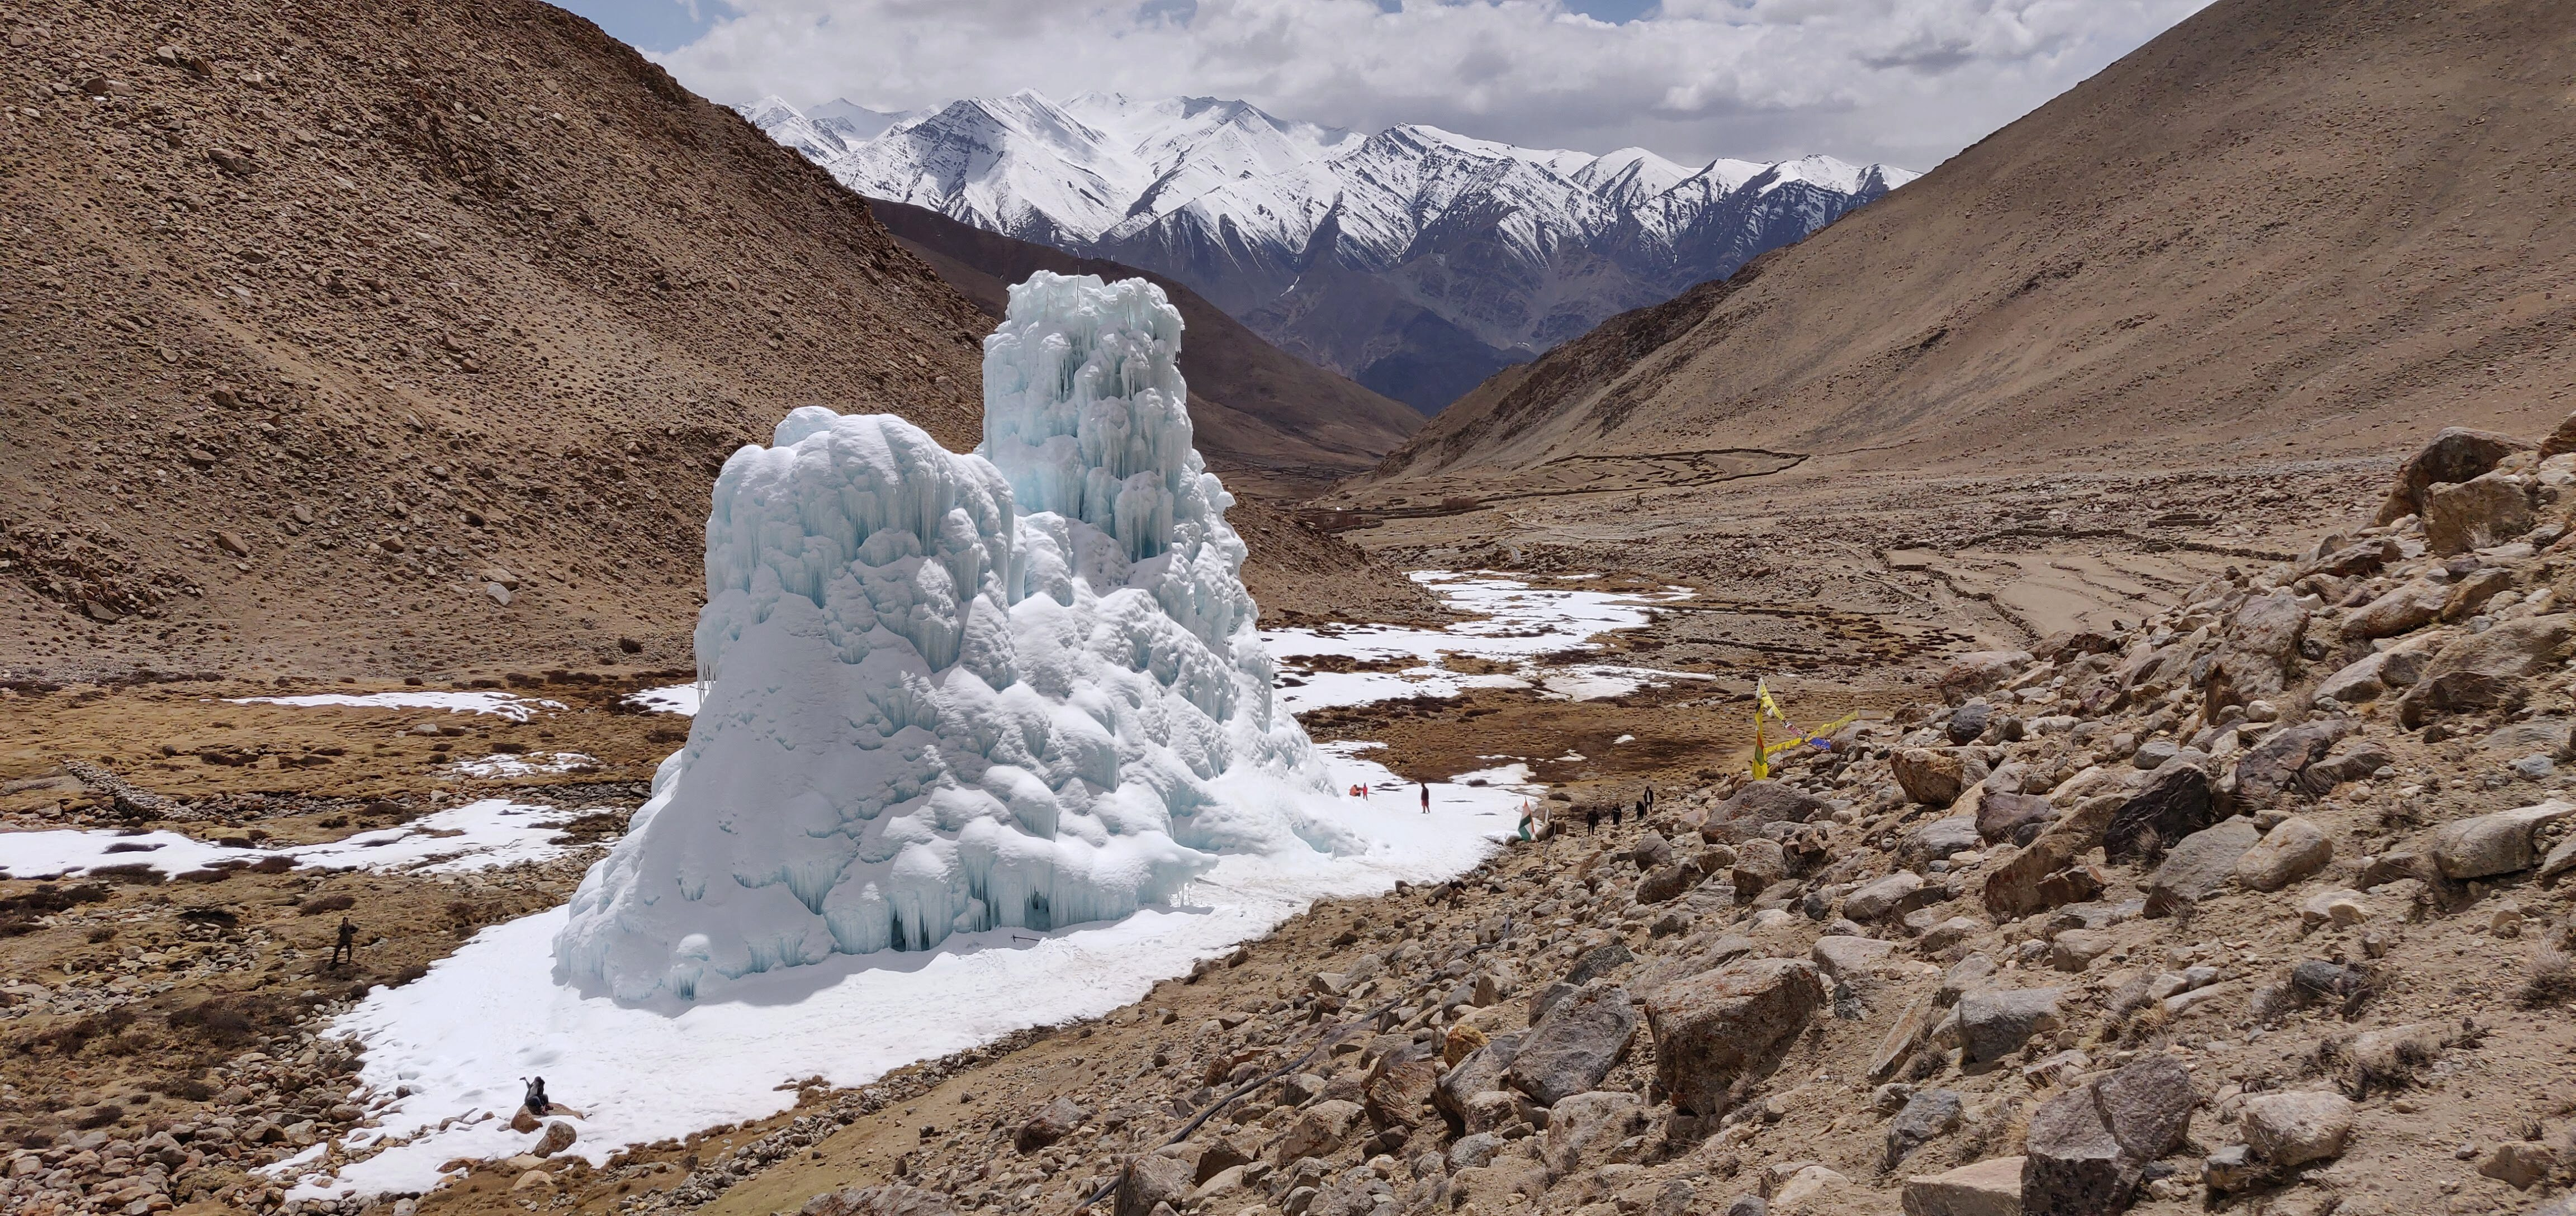
\includegraphics[width=12cm]{Figures/IS_example.jpg}

\caption{Ice terrace of Phuktse, viewpoint 4430 m. (a) February 2014 (b) October 2014 Adapted from: \cite{nusserSociohydrologyArtificialGlaciers2019}}

\label{fig:ISexample}
\end{figure}

\subsection{Drawbacks}

\section{Improvement of construction strategies through weather-sensitive automation systems}

\subsection{Perpetual ice reservoirs}

